%%=====================================================================================
%%
%%       Filename:  articulo.tex
%%
%%    Description:  Artículo
%%
%%        Version:  1.0
%%        Created:  10/03/2018
%%       Revision:  none
%%
%%         Author:  Herbert Arias (dayanqwe123@gmail.com), 
%%   Organization:  
%%      Copyright:  Copyright (c) 2018, Herbert Arias.
%%
%%          Notes:  
%%
%%=====================================================================================

\documentclass[twocolumns,a4paper]{IEEEtran}
\usepackage{graphicx}
\usepackage{amsmath}
\usepackage{authblk}
\usepackage[spanish]{babel}
\usepackage{blindtext}
\usepackage[utf8]{inputenc}
\usepackage{hyperref} 
\hypersetup{hidelinks}
\usepackage{csquotes} 
\usepackage[style=ieee]{biblatex} 
\bibliography{Bibliography.bib}

\graphicspath{{./pictures/}}

%%\title{Un breve recorrido por las tecnologías de Desarrollo Web en el 2018 }
\title{Rutas para el aprendizaje de tecnologías del desarrollo Web en la actualidad}

\author[1]{Herbert Brice Arias Silva}
\affil[1]{Departamento de Ingeniería de Software, Universidad Nacional Mayor de San Marcos}
\affil[2]{Introducción a las Ciencias e Ingeniería}

\begin{document}
\maketitle

\begin{abstract}
   En la actualidad la tecnología tiene un avance vertiginoso y esto genera
   mucho desconcierto al enfrentarse con la decisión de empezar el estudio de
   una de sus ramas, y este avance tiene un cambio mucho mayor en el ámbito de
   la informática ya que comunidades enteras de software así como empresas muy
   grandes del rubro están trabajando en el desarrollo de nuevas y mejoradas
   tecnologías que están reemplazando muy rápido a otras tecnologías
   consideradas nuevas y muy usadas años atrás. En este artículo se realiza un
   breve recopilatorio de esas tecnologías su origen y uso en la Programación
   Web, veremos en líneas generales un panorama de cómo un estudiante de
   primeros ciclos puede abarcar desde el inicio, una carrera profesional
   enfocada a la Programación Web y todo los conocimientos extras que implica
   adquirir a lo largo de su estudio universitario.
\end{abstract}

\section{Introducción}
Hoy en día casi para todo se requiere algún tipo de programación. Asi pues,
¿qué es?  Programar es básicamente explicarle a tu ordenador que quieres que
haga por ti.  Pero citemos lo que piensan sobre esto los grandes programadores
que han revolucionado algun sector con la programación:
\begin{itemize}
   \item Gabe Newell (creador de Valve): ``Cuando estás programando le estás
      enseñando a la cosa posiblemente más estúpida del universo, un ordenador,
      a hacer algo''.
   \item Mark Zuckerberg (creador de Facebook): ``Programar es una de las pocas
      cosas en el mundo que puedes hacer cuando estás sentado y simplemente
      crear algo completamente nuevo desde cero''
   \item Drew Houston (creador de Dropbox): ``Realmente no es muy diferente de
      tocar un instrumento o practicar un deporte. Empieza siendo algo muy
      intimidante, pero terminas por cogerle el truco.''
   \item Chris Bosh (programador de la NBA): ``Programar es algo que puede
      aprenderse. Y sé que puede ser intimidante, muchas cosas son
      intimidantes. Pero ya sabes ¿qué no lo es?''
\end{itemize}

La programación es algo absolutamente necesario en nuestra época, ya que está
en el centro de los mejores productos de la tierra, el software ya se apoderó
del mundo. Saber código hace a cualquier profesional mejor, ya que si un
profesional aprende a programar esto le dará una capacidad impresionante de
cambiar su profesión. Las personas más exitosas, la gente que tiene los
proyectos más exitosos grandes y de crecimiento en Internet son aquellos que
tienen la intersección de dos conocimientos y uno de esos conocimientos
necesarios en muchos de esos casos es la programación.

En el colegio hemos aprendido cosas muy complejas, y más para ingresar a la
universidad ya que se requieren tener cierto nivel de conocimientos complicados
como por ejemplo en química, balancear una ecuación por Redox o en física el
uso de ecuaciones para interpretar el movimiento parabólico de los cuerpos con
masa y aceleración... Entender los fundamentos de la programación es mucho más
sencillo que todo eso aunque aprender física o química incluso nos puede
acercar en cierto momento a querer aprender programación ya que aprender sobre
los semiconductores en química o los circuitos y teoría de transistores en
física nos acerca a la programación porque tienen mucho que ver. Pero ¿por qué
muchos sino la mayoría no aprendemos programación durante el colegio o más
crítico aún durante la universidad?. Esto tiene que ver con el Álgebra y el
cálculo, y es que con éstos saltamos a las matemáticas que casi siempre son
útiles para la Ingeniería Civil o para la ingeniería Bioquímica pero no
necesariamente para la Ingeniería de Sistemas, Ingeniería de Software o las
ciencias de la computación, por ejemplo nos enseñan límites, nos enseñan
integrales, nos enseñan a calcular el área bajo la curva, y es algo muy
importante pero a su vez es algo muy denso, es como si pasáramos de aprender a
conducir un automovil automático a aprender a conducir un automóvil de la
fórmula uno, y programar deja de ser prioridad en la vida universitaria de
muchos futuros ingenieros.

\begin{figure}[t!]
   \centering
   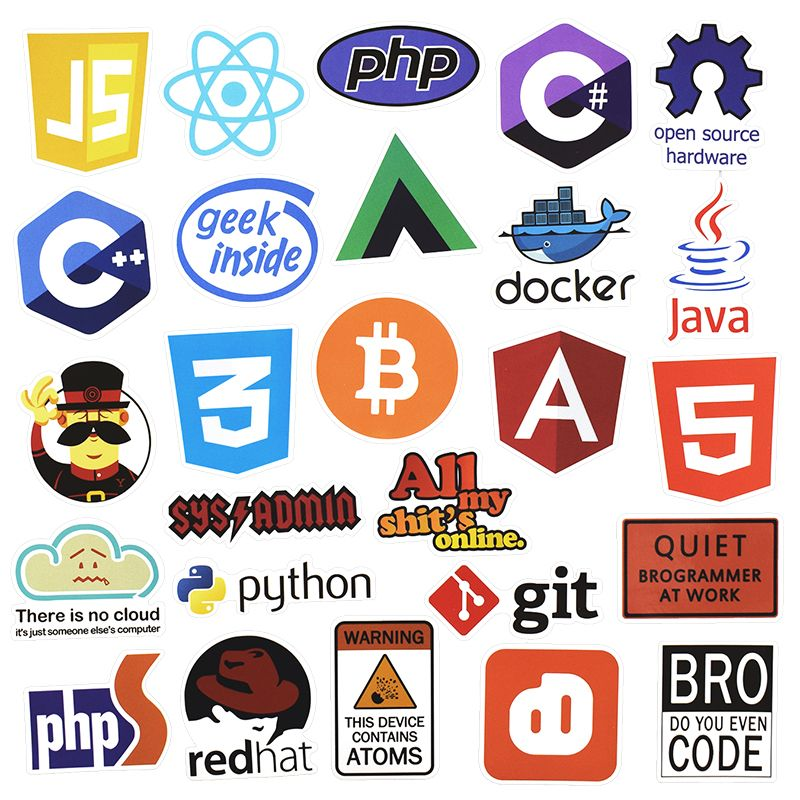
\includegraphics[width=2.5in]{tec_web}
   \caption{Lenguajes, sistemas y tecnologías Web}\label{ref:FiguraA}
\end{figure}

La mayor parte de la programación está relacionada con la Web y es que la
programación web es muy interesante y amplia, el hecho de que el lenguaje de
programación más popular y usado sea JavaScript, que es el lenguaje que nos
permite interactuar con los navegadores Web, no hace más que confirmar lo
anteriormente mencionado, es por ésto que es importante conocer un poco más la
esencia de la Web en la actualidad. Desde inicios del 2000 la web tuvo un punto
de quiebre y los cambios se visualizan en la actualidad ya que ahora se trata
de la Web Social o Web 2.0, donde destacan plataformas como Wikipedia, Youtube,
Facebook, Google, Flickr, Tumblr, Twitter, Instagram, Uber, etc. Y se tratan de
plataformas construidas para la gran masa de usuarios y son éstos los que crean
el contenido que otros consumen. Esta web está basado en dos princios:
\textbf{inteligencia colectiva} que es la suma del saber de cada uno de los
individuos que al compartirse puede dar lugar a una obra colectiva y la
\textbf{arquitectura de la participación} que implica una nueva forma de
construir los sitios web para permitir la participación de la gran masa de
usuarios. La web se convierte entonces en una plataforma de servicios donde los
usuarios asumen una filosofía que supone compartir los recursos propios a la
vez que nos beneficiamos de los ajenos, saldando así una especie de deuda con
la comunidad.\cite{NataliaVazquezWeb2007}.

El objetivo principal de este breve artículo no es solo el de informar qué
tecnologías web son a las que podemos apuntar aprender sino el de instar a
formular proyectos desde ahora ya que el camino de la programación Web implica
adquirir conocimientos, pero más importante aplicarlos y en el camino descubrir
qué nuevos conocimientos podemos y debemos adquirir.

Inicialmente el artículo busca motivar a mis compañeros a involucrarse con el
desarrollo Web y que conozcan las herramientas y tecnologías así como recursos
de aprendizaje a la que todos podemos acceder ya que el Internet es libre, pero
muchas veces no conocemos los recursos y no logramos encontrarlos y
aprovecharlos.

\section{Antecedentes}






















\section{Requerimientos necesarios}
Al formarse como programador Web es necesario escoger una ruta, ya que para
dedicarse a esta rama de la informática incluso hay que especializarse. Se
puede elegir entre dos caminos o rutas: Fronted y Backend, pero antes de entrar
en detalle de estas dos ruta es necesario conocer algunas herramientas y
fundamentos que nos ayudarán sin importar cual sea el camino que hayamos
elegido.
\subsection{Git - Sistema de control de versiones}
\cite{pascual199012}\cite{mycite2016}\cite{Chavez-Campos2016}\cite{webdev:2018:online}\cite{SergioLujan2001}\cite{NataliaVazquezWeb2007}\cite{WebDev:2018:online}\cite{ScottBenGit2014}\cite{Ssh:2018:online}\cite{HTTP:2018:online}\cite{HTTPS:2018:online}\cite{ChrisNegusLinux2005}\cite{JoyanesProg2008}\cite{GuidesGitHub:2018:online}\cite{HTMLw3:2018:online}\cite{PluralsightJavaScript:2018:online}\cite{JavaScriptw3:2018:online}\cite{PythonTuto:2018:online}\cite{IntroPython2008}


\printbibliography
\end{document}
